\documentclass[12pt]{article}
\usepackage[utf8]{inputenc}

\usepackage{lmodern}

\usepackage{enumitem}
\usepackage[margin=2cm]{geometry}

\usepackage{amsmath, amsfonts, amssymb}
\usepackage{graphicx}
%\usepackage{subfigure}
\usepackage{tikz}
\usepackage{pgfplots}
\usepackage{multicol}

\usepackage{comment}
\usepackage{url}
\usepackage{calc}
\usepackage{subcaption}
\usepackage[indent=0pt]{parskip}
\usepackage{animate}

\usepackage{array}
\usepackage{blkarray,booktabs, bigstrut}
\usepackage{bigints}

\pgfplotsset{compat=1.16}

% MATH commands
\newcommand{\ga}{\left\langle}
\newcommand{\da}{\right\rangle}
\newcommand{\oa}{\left\lbrace}
\newcommand{\fa}{\right\rbrace}
\newcommand{\oc}{\left[}
\newcommand{\fc}{\right]}
\newcommand{\op}{\left(}
\newcommand{\fp}{\right)}

\newcommand{\bi}{\mathbf{i}}
\newcommand{\bj}{\mathbf{j}}
\newcommand{\bk}{\mathbf{k}}
\newcommand{\bF}{\mathbf{F}}

\newcommand{\mR}{\mathbb{R}}

\newcommand{\ra}{\rightarrow}
\newcommand{\Ra}{\Rightarrow}

\newcommand{\sech}{\mathrm{sech}\,}
\newcommand{\csch}{\mathrm{csch}\,}
\newcommand{\curl}{\mathrm{curl}\,}
\newcommand{\dive}{\mathrm{div}\,}

\newcommand{\ve}{\varepsilon}
\newcommand{\spc}{\vspace*{0.5cm}}

\DeclareMathOperator{\Ran}{Ran}
\DeclareMathOperator{\Dom}{Dom}

\newcommand{\exo}[1]{\noindent\textcolor{red}{\fbox{\textbf{Problem {#1}}}\hrulefill}\\\\ }
\newcommand{\qu}[4]{\noindent\textcolor{#4}{\fbox{\textbf{Section {#1} | Problem {#2}}} \hrulefill{{\fbox{\textbf{{#3} Points}}}}\\}}

\newcommand{\semester}{Fall 2023}

\newcommand{\CVup}{%

\begin{tikzpicture}
\draw[black, <->, >=latex] (-0.33, 0.5) .. controls (-0.125, 0) and (0.125, 0) .. (0.33, 0.5);
\end{tikzpicture}}

\newcommand{\CVupInc}{%
\begin{tikzpicture}
\draw[black, ->, >=latex] (0,0) .. controls (0.2, 0) and (0.4, 0.2) .. (0.5, 0.5);
\end{tikzpicture}}

\newcommand{\CVupDec}{%
\begin{tikzpicture}[rotate=270]
\draw[black, ->, >=latex] (0,0) .. controls (0.2, 0) and (0.4, 0.2) .. (0.5, 0.5);
\end{tikzpicture}}

\newcommand{\CVdown}{%
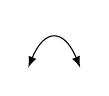
\begin{tikzpicture}
\draw[black, <->, >=latex] (-0.33, -0.5) .. controls (-0.125, 0) and (0.125, 0) .. (0.33, -0.5);
\end{tikzpicture}}

\newcommand{\CVdownInc}{%
\begin{tikzpicture}
\draw[black, ->, >=latex] (-0.5, -0.5) .. controls (-0.5, -0.3) and (-0.5, -0.1) .. (0,0);
\end{tikzpicture}}

\newcommand{\CVdownDec}{%
\begin{tikzpicture}[rotate=-90]
\draw[black, ->, >=latex] (-0.5, -0.5) .. controls (-0.5, -0.3) and (-0.5, -0.1) .. (0,0);
\end{tikzpicture}}

\begin{document}
	\noindent \hrulefill \\
	MATH-244 \semester \hfill Practice Problems Solutions\\
	Section 15.3 \hfill Pierre-Olivier Paris{\'e} \\\vspace*{-1cm}
	
	\noindent\hrulefill
	
	\spc

	\underline{\textsc{Practice Problems from Section 10.3}}

	\exo{4}
	\vspace*{-0.5cm}
	\begin{enumerate}[label=\alph*)]
		\item $r = 4$ and $\theta = 3\pi / 4$. So $x = 4 \cos (3 \pi /4) = 4 (-\sqrt{2}/2) = -2 \sqrt{2}$ and $y = 4 \sin (3 \pi / 4) = 4 (\sqrt{2} / 2) = 2 \sqrt{2}$.
		\item $r = \sqrt{2}$ and $\theta = \pi /4$. So $x = \sqrt{2} \cos (\pi /4) = 2$ and $y = \sqrt{2} \sin (\pi /4 ) = 2$.
	\end{enumerate}	

	\exo{6(i)}
	\vspace*{-0.5cm}
	\begin{enumerate}[label=\alph*)]
		\item $x = -4$ and $y = 4$, so $r = \sqrt{(-4)^2 + (4)^2} = \sqrt{32} = 4 \sqrt{2}$ and $\theta = \arctan (4 / -4) = \arctan (-1) = - \pi / 4 + k \pi$, where $k$ is an integer. However, $x < 0$ and $y >0$, so the point $(x, y)$ should be in the second quadrant. Therefore, the angle is $\theta = -\pi/ 4 + \pi = 3\pi /4$.
		\item $x = 3$ and $y= 3 \sqrt{3}$, so $r = \sqrt{9 + 9 \cdot 3} = \sqrt{36} = 6$ and $\theta = \arctan (\frac{1}{\sqrt{3}}) = \pi / 6 + k \pi$, where $k$ is an integer. However, $x > 0$ and $y > 0$, so the point $(x, y)$ should be in the second quadrant. Therefore, the angle is $\theta = \pi / 6$. 
	\end{enumerate}

	\exo{16}
	\\
	We have $\sec \theta = 1/ \cos \theta = 1/ (x/r) = r /x$ because $\cos \theta = x/r$. Therefore, the polar equation becomes $\sqrt{x^2 + y^2} = \frac{4\sqrt{x^2 + y^2}}{x}$.Dividing by $\sqrt{x^2 + y^2}$, we get
		\begin{align*}
		1 = \frac{4}{x} .
		\end{align*}
	which means $x = 4$. This is a vertical line.

	\exo{17}
	\\
	We have $r = \sqrt{x^2 + y^2}$ and $\cos \theta = \frac{x}{r}$, so that
		\begin{align*}
		r = 5 \frac{x}{r} \quad \Ra \quad r^2 = 5x \quad \Ra \quad x^2 + y^2 = 5x .
		\end{align*} 
	After simplifications, we get $(x - 5)^2 + y^2 = 25$ and this is a circle of radius $5$ and centered at the point $(5, 0)$.

	\vspace*{1cm}

	\underline{\textsc{Practice Problems from Section 15.3}}

	\exo{12}
	\\
	Let $x = r \cos \theta$ and $y = r \sin \theta$ (we change from cartesian to polar coordinates). The equation of the circle of radius $2$ centered at the origin is simply $r = 2$. Also, in polar coordinates, we have $dA = r dr d\theta$ and so
		\begin{align*}
		\iint_D \cos \sqrt{x^2 + y^2} \, dA = \int_0^{2\pi} \int_0^2 (\cos r) r \, dr d\theta = \Big( \int_0^{2\pi} \, d\theta \Big) \Big( \int_0^2 r \cos r \, dr \Big) .
		\end{align*}
	After an integration by parts, the value of the integral is
		\begin{align*}
		\iint_D \cos \sqrt{x^2 + y^2} \, dA = 2\pi (-1 + 2 \sin (2) + \cos (2) ) .
		\end{align*}
	
	\spc
	
	\exo{16}
	\\
	We draw the region between the two cardioids. Here are the two regions (in green) enclosed within the two cardiods:
		\begin{figure}[h]
		\centering
		\includegraphics[scale=0.3]{exo-16_15-3.png}
		\end{figure}
	The two cardiods meet when $1 + \cos \theta = 1 - \cos \theta$. After rearranging, we have to solve the equation $2 \cos \theta = 0$. This occurs only when $\theta$ is $\pi/2 + k \pi$. We choose the values $\theta = \pi/2$ and $\theta = -\pi/2$. So, the polar coordinates of the two points of intersection are
		\begin{align*}
		(1, \pi/2 ) \quad \text{ and } \quad (1, -\pi/2)
		\end{align*}
	which corresponds to the following points in the cartesian plane:
		\begin{align*}
		(0, 1) \quad \text{ and } \quad (0, -1 ). 
		\end{align*} 
		
	We have now to setup the integral. Let $D$ denote the region enclosed by the two cardioids. The area is given by
		\begin{align*}
		A (D) = \iint_D \, dA .
		\end{align*}
	In polar coordinates, we have $dA = r dr d\theta$. Due to the symmetry of the domain, we can only compute the area of the petal with a positive (or zero) $y$ coordinate (above the $x$-axis) and then multiply our result by $2$. Call this region $D_1$. 
	
	The argument $\theta$ will vary from $0$ to $\pi$. However, we have to split the interval $[0, \pi]$ into the intervals $[0, \pi/2]$ and $[\pi/2, \pi ]$ because the cardioids intersect at $\theta = \pi/2$. We can apply again the symmetry argument because the region $D_1$ is symmetric with respect to the $y$ axis and multiply by $2$ to get the area of $D_1$. Denote half of the petal by $D_2$. So we have
		\begin{align*}
		A(D_2) = \int_0^{\pi/2} \int_0^{\textcolor{blue}{1 - \cos (\theta )}} r \, dr d\theta = \int_0^{\pi/2} \frac{(1 - \cos \theta )^2}{2} \, d\theta = \frac{3 \pi}{8} - 1 .
		\end{align*}
	Thus, 
		\begin{align*}
		A (D) = 2 A(D_1) = 4 A(D_2) = \frac{3\pi}{2} - 4 .
		\end{align*}

	\spc 

	\exo{22}
	\\
	The surfaces that bounds the $z$-coordinate are $z = \sqrt{16 - x^2 - y^2}$ and $z = -\sqrt{16 - x^2 - y^2}$. We want the solid outside the cylinder $x^2 + y^2 = 2^2$. Let $D$ be the domain of integration, then the volume of the solid is given by
		\begin{align*}
		V(S) = \iint_D \sqrt{16 - x^2 - y^2} - (- \sqrt{16 - x^2 - y^2}) \, dA = \iint_D 2 \sqrt{16 - x^2 - y^2} \, dA .
		\end{align*}
	
	To find $D$, we will project on the $XY$-plane. The projections of the cylinder on the $XY$-plane is a circle of radius $2$ and the projection of the sphere on the $XY$-plane is a circle of radius $4$. Thus we want the region between these two circles.
		\begin{figure}[h]
		\centering
		\includegraphics[scale=0.3]{exo22_15-3.png}
		\end{figure}
	We will change in polar coordinates. The equation of the two circles are $r = 2$ and $r = 4$ and the angle ranges from $0$ to $2\pi$. So, in polar coordinates, we have
		\begin{align*}
		D = \{ (r, \theta ) \, : \, 2 \leq r \leq 4 \text{ and } 0 \leq \theta \leq 2\pi \} .
		\end{align*}
		
	Thus, using the change of variable formula, we get
		\begin{align*}
		V(S) = 2 \int_{0}^{2\pi} \int_2^4 (\sqrt{16 - r^2}) r \, dr d\theta = 4\pi \int_2^4 r \sqrt{16-r^2} \, dr .
		\end{align*}
	Setting $u = 16 - r^2$ and completing the calculations for the integral, we get the value 
		$$
		V(S) = 32 \pi \sqrt{3} .
		$$
	
	\spc
	
	\exo{32}
	\\
	The bounds in the integrals give us
		\begin{align*}
		D = \{ (x, y) \, : \, 0 \leq x \leq 2 \text{ and } 0 \leq y \leq \sqrt{2x - x^2} \}
		\end{align*}
	So, the upper bound of $y$ is half of a circle of radius $1$ and center $(1, 0)$ because
		\begin{align*}
		y = \sqrt{2x - x^2} \iff (x-1)^2 + y^2 = 1 .
		\end{align*}
	So the region looks like this
		\begin{figure}[h]
		\centering
		\includegraphics[scale=0.5]{exo32-15-3.png}
		\end{figure}
		
	Let's describe the domain $D$ in polar coordinates. Let $x = r\cos \theta$ and $y = r \sin \theta$. The equation of the circle in polar coordinate is $r = 2\cos \theta$ (replace $x$ and $y$ by $r\cos \theta$ and $r\sin \theta$ in the equation $x^2 + y^2 = 2x$). Also, the angle $\theta$ will vary from $0$ to $\pi/2$ so we cover the upper half of the circle (and its interior). So
		\begin{align*}
		D = \{ (r, \theta ) \, : \, 0 \leq r \leq 2\cos \theta \text{ and } 0 \leq \theta \leq \pi/2 \} .
		\end{align*}
		
	We can now compute the integral, call it $I$, in polar coordinates:
		\begin{align*}
		I = \int_0^{\pi/2} \int_0^{2\cos \theta} r^2 \, dr d\theta = \frac{8}{3} \int_0^{\pi/2} \cos^3 \theta \, d \theta = \frac{2}{3} \int_0^{\pi/2} 3 \cos (\theta ) + \cos (3\theta ) \, d\theta .
		\end{align*}
	After finding the value of the integral, we get $I = 16/9$.

\end{document}